
\chapter{TINJAUAN PUSTAKA}

\section{Landasan Teori}

\subsection{Citra Digital}
Citra digital merupakan representatif dari citra yang diambil oleh \textit{device} dengan bentuk pendekatan berdasarkan sampling dan kuantisasi. Sampling menyatakan besarnya kotak-kotak yang disusun dalam baris dan kolom. Dengan kata lain, sampling pada citra menyatakan besar kecilnya ukuran pixel pada citra, dan kuantisasi menyatakan besarnya nilai tingkat kecerahan yang dinyatakan dalam nilai tingkat keabuan sesuai dengan jumlah bit biner yang digunakan oleh \textit{device} yang digunakan. 

Citra digital dapat didefinisikan sebagai fungsi f(x,y) berukuran M baris dan N kolom, dengan x dan y adalah kordinat spasial, dan amplitudo f di titik kordinat (x,y) dinamakan intensitas atau tingkat keabuan dari citra pada citra tersebut (\cite{book:darma}). Berdasarkan jenis warnanya citra digital dibagi menjadi 3 jenis:

\begin{itemize}
    \item \textbf{Citra Biner (Monokrom)}, Banyaknya dua warna, yaitu hitam dan putih. Warna hitam direpresentasikan dengan 1 dan warna putih direpresentasikan dengan 0. Dibutuhkan 1 bit di memori untuk menyimpan warna ini.
    \item \textbf{Citra Grayscale (Skala keabuan)}, Banyaknya warna tergantung pada jumlah bit yang disediakan di memori untuk menampung kebutuhan warna ini. Citra 2 bit mewakili 4 warna, citra 3 bit mewakili 8 warna, dan seterusnya. Semakin besar jumlah bit warna yang disediakan di memori, semakin halus gradasi warna yang terbentuk. Pada umumnya citra digital grayscale menggunakan 8 bit memori dengan derajat keabuan dari 0 sampai 255.
    \item \textbf{Citra Warna}, Setiap piksel pada citra warna mewakili warna yang merupakan kombinasi dari tiga warna dasar (RG8 = Red Green Blue). Setiap warna dasar menggunakan penyimpanan 8 bit, yang berarti setiap warna mempunyai gradasi sebanyak 255 warna. Berarti setiap piksel mempunyai kombinasi warna sebanyak 255 x 255 x 255 =16 juta warna lebih. Dibutuhkan 3x8 = 24 bit di memori untuk menyimpan sebuah data warna ini.
\end{itemize}

\subsection{Video Streaming}
\blindtext

\subsection{FPGA}
Field Programmable Gate Arrays atau FPGA adalah perangkat semikonduktor yang berbasis \textit{matriks configurable logic block} (CLBs) yang terhubung melalui interkoneksi yang dapat diprogram.

FPGA dapat diprogram ulang ke aplikasi atau fungsi yang diinginkan setelah \textit{manufacturing}. Fitur ini yang membedakan FPGA dengan \textit{Application Specific Integrated Circuits} (ASICs), yang dibuat khusus untuk tugas tertentu saja (\cite{XILINX}).

Sebuah \textit{microprocessor} menerima instruksi berupa kode 1 atau 0, kode-kode ini selanjutnya diinterpretasikan oleh komputer untuk menjalankan perintah yang diberikan. \textit{Microprocessor} ini membutuhkan intruksi berupa kode secara terus menerus untuk menjalankan fungsinya. Sedangkan pada FPGA hanya dibutuhkan sekali konfigurasi \textit{chip} setiap kali dinyalakan. Membuat atau mengunduh \textit{bitstream} yang menentukan fungsi logika dilakukan oleh \textit{logic elements} (LEs), sebuah sirkuit dapat dibuat dengan mengabungkan beberapa LEs menjadi satu kesatuan. Setelah \textit{bitstream} dipasang, FPGA tidak perlu lagi membaca instruksi berupa 1 dan 0, berbeda dengan \textit{microprocessor} yang selalu membutuhkan instruksi (\cite{pdf:cheung}).

\begin{afigure}{Struktur FPGA}
    \label{fig:fpga-structure}
    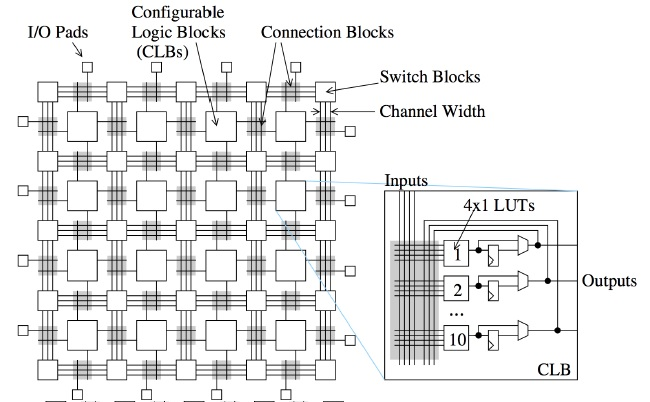
\includegraphics[width=12cm, center]{images/fpga-structure.jpeg}
\end{afigure}



\subsection{Tepi Citra}
Suatu titik (x, y) pada citra digital dikatakan sebagai tepi apabila perubahan nilai intensitas derajat keabuan yang mendadak (besar) dalam jarang yang berdekatan. Tepi biasanya terdapat pada batas andara dua daereah yang berbeda pada suatu citra. Tepi pada citra dapat merepresentasikan objek-objek yang terkandung dalam citra tersebut, bentuk dan ukurannya atau terkadang juga informasi tentang teksturnya.

Tepi citra dapat dilihat melalui perubahan intensitas pixel pada suatu area. Berdasarkan perbedaan perubahan intensitas tersebut, tepi dapat dibagi menjadi 4 jenis yaitu tepi steep, ramp, line dan step-line (\cite{book:darma}).

\subsubsection{Step}
Tepi jenis \textit{step} merupakan tepi citra yang berbentuk dari perubahan intensitas nilai pixel secara signifikan dari tinggi ke rendah ataupun sebaliknya.
% Tambahkan gambar 

% halaman 201
% https://books.google.co.id/books?hl=en&lr=&id=NectMutqXJAC&oi=fnd&pg=PR4&dq=buku+pengolahan+citra+digital&ots=C2oB2TDTo4&sig=UnkxuezGlrECiOZBepXOMa__gEY&redir_esc=y#v=onepage&q=buku%20pengolahan%20citra%20digital&f=false

\subsubsection{Ramp}
Tepi jenis ini terbentuk dari perubahan intensitas nilai pixel secara perlahan. Perubahan secara perlahan dapat dilihat pada bentuk kurva yang semakin tinggi dengan perubahan kontinu.

\subsubsection{Line}
Tepi jenis ini ditandai dengan perubahan intensitas nilai pixel secara drastis dari rendah-tinggi-rendah atau sebaliknya.

\subsubsection{Step-line}
Tepi \textit{step-line} merupakan gabungan dari tepi jenis step dan line. Tepi jenis ini ditandai dengan peningkatan intensitas yang tajam dalam interval tertentu dan kemudian ditandai dengan penurunan yang tidak signifikan, sehingga perubahan intensitas nilai pixel selanjutnya berlangsung stabil.


\subsection{Deteksi Tepi}
Deteksi tepi merupakan salah satu metode dalam pemrosesan cira digital untuk deteksi fitur dan ekstraksi dengan mengidentifikasi titik-titik (pixel) dalam citra yang mengalami perubahan tingkat keabuan secara derastis dan mengalami diskontinu. Salah satu tujuan deteksi tepi yaitu untuk mengurangi jumlah data secara signifikan dalam suatu gambar dan mempertahankan sifat strukturalnya untuk pemrosesan citra lebih lanjut. (\cite{desi_herawati}).

Berbagai macam metode deteksi dapat digunakan untuk mendeteksi tepi pada citra. Setiap teknik memiliki keunggulan dan karakteristiknya masing-masing. Suatu teknik deteksi tepi mungkin dapat bekerja sangat baik dalam suatu aplikasi tertentu namun sebaliknya belum tentu dapat berjalan secara maksimal pada aplikasi lainnya.

Terdapat berbagai operator deteksi tepi yang telah dikembangkan berdasarkan turunan pertama (first order derrivate), di antaranya operator Robert, operator Sobel, operator Prewitt, operator Krisch, dan operator Canny. Konsep dasar dari deteksi tepi dengan turunan pertama adalah dengan memanfaatkan perbedaan nilai suatu pixel dengan pixel tetangganya. 
% operator turunan kedua, dan seterusnya

\subsection{Pengolahan Citra Digital}
sesuatu (\cite{book:gonzalez})

\section{Penelitian Terkait}
\subsection{Spatial Filtering Based Boundary Extraction in Underwater Images for Pipeline Detection: FPGA Implementation}
\blindtext (\cite{soa:alex-raj})

\subsection{FPGA Implementation of Spatial Filtering techniques for 2D Images}
\blindtext (\cite{soa:sushant})

\subsection{Features of Image Spatial Filters Implementation on FPGA}
\blindtext (\cite{soa:dmitry})

\subsection{An FPGA-Oriented Algorithm for Real-Time Filtering of Poisson Noise in Video Streams, with Application to X-Ray Fluoroscopy}
\blindtext (\cite{soa:castellano})

\subsection{A real-time video denoising algorithm with FPGA implementation for Poisson–Gaussian noise}
\blindtext (\cite{soa:xin})